\maketitle

\begin{abstract}
Conversational memory systems select sessions $K$ and a per-session context budget $B$. We derive an oracle ceiling on recovering every labeled evidence session in LongMemEval --- a dataset property before text truncation, not operating guidance. The smallest depth reaching 99.5\% coverage is $K^*=6$ on both cleaned scales, which share their evidence counts. At $K=1$, the ceiling is 100\% for single-session questions and 0\% for multi-session or knowledge-update questions. A protocol-specified crossed depth--budget GEE remains unexecuted. An exploratory Gemma-4-E4B-it pilot ran 18 conditions; 17 refusals triggered a coverage gate (single-reader NO-GO) that stopped advancement. Excluding 540 unanswerable trials and 16 answerable refusals left 8,444 trials; exact match was 6.71\%. The budget association was positive ($\hat\beta_B=0.3166$ log-odds, $p=2.46\times10^{-4}$) and the interaction inconclusive ($\hat\beta_{KB}=0.0111$, 95\% CI $[-0.0217,0.0439]$). Strict full-string exact match can reward longer outputs under larger budgets, so this exploratory, single-reader association cannot be attributed to evidence quality alone. Across 9,004 latency records the pooled 95th-percentile generation time was 15.72~s on a laptop GPU; the crossed $K\ge4$, $B=512$ tail was 26.15~s. Coverage, scoring, and latency must be measured together.
\end{abstract}

\begin{IEEEkeywords}
Agent memory, retrieval-augmented generation, LongMemEval, factorial design, generalized estimating equations.
\end{IEEEkeywords}

\section{Introduction}

Conversational agents can retrieve evidence from past interactions instead of passing every turn to a language model~\cite{lewis2020rag,packer2023memgpt}. On LongMemEval, Wu et~al. reported large accuracy drops for long-context models given full histories compared with gold evidence alone~\cite{wu2025longmemeval}. Here $K$ counts ranked multi-turn sessions, and $B$ is the nominal budget per retained session. The product $KB$ approximates the maximum evidence budget. The same product can represent four sessions with $B=512$ or thirty-two sessions with $B=64$, with different evidence coverage and within-session detail.

We ask how much labeled evidence can fit at a given depth and whether the association between depth and answer accuracy changes with the per-session budget. The first question has an oracle answer from benchmark metadata. For the second, we specify a crossed design and report a single-reader exploratory pilot. The pilot estimates associations for one configuration and identifies constraints on a multi-reader study.

\section{Related Work}

\textit{Memory evaluation.} LongMemEval, LoCoMo, and LiCoMemory evaluate different facets of long-term conversational memory~\cite{wu2025longmemeval,maharana2024locomo,huang2026licomemory}. Yuan et~al. diagnose retrieval versus utilization bottlenecks in agent memory~\cite{yuan2026diagnosing}. Shao et~al. evaluate stored-evidence usability conditioned on corpus scale~\cite{shao2026storedevidence}. Shen audits forgetting with a restore counterfactual~\cite{shen2026evictiondestroys}. MemTier and a LightMem reproduction examine tiered memory and retrieval or construction choices~\cite{sidik2026memtier,zhou2026reproducinglightmem}. Diagnostic studies cover operation-level evaluation, write/retrieval bottlenecks, and budget-dependent operator selection~\cite{liu2026evalmem,yu2026whenloss,kang2026retainconsolidate}. Andreev evaluates depth and reconstructed context width in hierarchical retrieval~\cite{andreev2026depthwidth}. MemSat varies the \emph{count of retrieved sessions} and the \emph{budget per session} on LongMemEval, pairing that design with an oracle bound on complete session recovery.

\textit{Count, length, and reader effects.} Levy et~al. isolate the challenge of multiple documents at fixed context length~\cite{levy2025moredocuments}. Along $L=KB$, the derivative of a performance surface is $\partial y/\partial K-(L/K^2)\partial y/\partial B$. The crossed grid estimates separate slopes and their interaction. Position and irrelevant context can affect reader accuracy~\cite{liu2024lostmiddle,hong2025contextrot}. A systems-level analysis examines sensitivity, robustness, and stability in retrieval-augmented generation~\cite{systems2026ragstability}. Fixed RAG compression can distort reader comparisons, and memory evaluations can vary across readers and judging setups~\cite{panthi2026fixedrag,chanhnourack2026auditing}. Statistical generalizability and observer-agreement measurement motivate an in-domain reliability audit~\cite{liu2025kappa0118,landis1977measurement}.

\textit{Routing and systems.} BudgetMem learns query-conditioned runtime budget tiers~\cite{zhang2026budgetmem}. MemGPT uses operating-system abstractions for context management~\cite{packer2023memgpt}. The oracle ceiling is a pre-truncation diagnostic of dataset metadata: it counts labeled sessions, not packed-prompt evidence or reader use. By analogy with Denning's working set size (WSS)~\cite{denning1968workingset}, a question with $m$ gold sessions needs at least $m$ resident slots: below that depth the missing sessions cannot enter the prompt at any per-session budget, the analogue of thrashing when the working set does not fit memory. This is a retrieval-side bound, not operating guidance; useful depths also depend on retrieval quality, truncation, and reader behavior.

\section{Oracle Recall Ceiling}
\label{sec:ceiling}

Let $\mathcal Q$ be the 470 answerable questions in the cleaned benchmark, excluding 30 unanswerable questions. Let $N_q$ be the history sessions and $S_q\subseteq N_q$ the distinct gold sessions from \texttt{answer\_session\_ids}. A top-$K$ set can contain every gold session only if $|S_q|\le K$. An oracle achieves that coverage by selecting gold sessions first. The complete-recall ceiling and its saturation depth at tolerance $\epsilon=0.005$ are
\begin{align}
C(K) &= |\mathcal Q|^{-1}\sum_{q\in\mathcal Q}\mathbf{1}[|S_q|\le K], \\
K^* &= \min\{K\in\mathbb N:C(K)\ge 1-\epsilon\}.
\end{align}
For mean partial recall, the corresponding ceiling is $P(K)=|\mathcal Q|^{-1}\sum_q\min(1,K/|S_q|)$. Both ceilings concern the retrieval of session IDs before text truncation.

\subsection{Scale and question type}

The cleaned S and M scales have the same 470 answerable questions and the same per-question gold-session counts. Wu et~al. report evidence spanning up to six sessions~\cite{wu2025longmemeval}. The counts for one through six gold sessions in our answerable subset are 170, 229, 39, 18, 11, and 3. Thus $C(K)$ is 36.17\%, 84.89\%, 93.19\%, 97.02\%, 99.36\%, and 100\% at depths one to six. The dataset-specific ceiling reaches $K^*=6$ on both scales even though median histories contain 47 and 476 sessions, respectively.

At $K=1$, the ceiling reaches 100\% for single-session assistant ($n=56$), user ($n=64$), and preference ($n=30$) questions. It reaches 15.75\% for temporal reasoning ($n=127$), and 0\% for multi-session ($n=121$) and knowledge-update ($n=72$) questions. Zero complete recall still permits the recovery of some gold sessions. By question type, the oracle ceiling $C_t(K)$ rises with depth: $C_t(2)=61.98\%$ and $C_t(4)=95.04\%$ for multi-session questions, and $C_t(2)=100\%$ for knowledge-update questions. Since observed multi-session exact match stays at or below $1.11\%$ through $K=32$, by $K=4$ the residual deficit is reader-side rather than retrieval-side, although budget truncation remains uncontrolled. The fraction of histories for which $K$ can reach every session,
\begin{equation}
D(K)=|\mathcal Q|^{-1}\sum_{q\in\mathcal Q}\mathbf{1}[K\ge |N_q|],
\end{equation}
is 100\% on S and 0\% on M at $K=64$. This boundary concerns session selection, before any budget truncation.

\begin{figure}[!t]
\centering
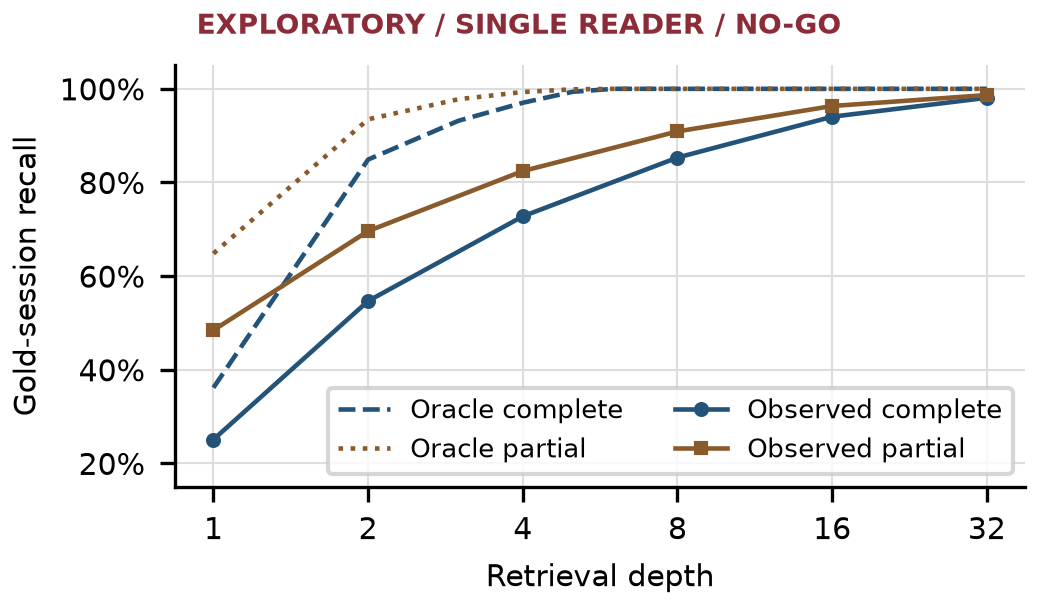
\includegraphics[width=\linewidth]{figures/fig1_recall_ceiling_vs_observed.png}
\caption{Analytic recall ceiling $C(K)$ (dashed) versus observed retriever recall across $K\in\{1,2,4,8,16,32\}$ on LongMemEval-S ($n=470$ answerable items). The ceiling saturates at $K^*=6$ ($100\%$) on both cleaned scales. The inset shows stratified recall: single-session items reach $98.2\%$ at $K=1$, while multi-session items rise from $35.9\%$ at $K=1$ to about $99.0\%$ at $K=32$. Status: ANALYTIC - DATASET PROPERTY for the ceiling curves; the observed retriever overlay is pilot data, and the embedded image watermark is unchanged.}
\label{fig:ceiling_vs_observed}
\end{figure}

Observed mean partial recall increased from 48.45\% at $K=1$ to 82.44\%, 96.33\%, and 98.67\% at $K=4,16,32$, respectively (Fig.~\ref{fig:ceiling_vs_observed}). At $K=32$, complete recall was 98.09\%. Recovery of a labeled session before truncation leaves open whether the packed prompt contains the answer evidence; the gap between the $100\%$ oracle ceiling reached by $K=6$ and $98.09\%$ observed complete recall at $K=32$ reflects imperfect retrieval together with budget truncation, neither of which the oracle model represents.

\section{Planned Confirmatory Design}
\label{sec:design}

The versioned protocol records the intended hypothesis and lists guide sign-off as pending. Formal preregistration would fix the analysis choices before the confirmatory run~\cite{article2018preregistration}. The configured grid crosses $K\in\{1,2,4,8,16,32\}$ and $B\in\{128,256,512\}$ on S and M with three planned readers (Gemma-4-E4B-it, Qwen3.5-9B, and Phi-4-mini-instruct) and three repetitions per question and cell. This gives 108 nominal reader--scale--factor cells. The power calculation used the 54-cell common-support rectangle with $K\in\{1,2,4\}$ and the three $B$ values. Under its simulation assumptions, the interaction minimum detectable effect (MDE) for that design was 0.0308 log-odds at 80\% power and $\alpha=0.05$. Hardware support still needs to be measured for the final panel. The plan calls for two sequential judges and an agreement audit on the study's own items. Before any headline parameters are reported, the protocol requires inter-judge agreement on the study's own items to clear a preregistered floor of Cohen's $\kappa\ge0.118$, slight agreement on the Landis--Koch scale~\cite{landis1977measurement}. The prospective gate is motivated by audits in which re-judging byte-identical responses flipped verdicts; the gate binds the planned run, not this exploratory pilot. The confirmatory experiment remains unexecuted.

\subsection{Model and estimand}

Let $x$ and $z$ denote $\log_2 K$ and $\log_2 B$, centered over the distinct grid levels. The proposed population-averaged GEE uses question-level clusters, independence working correlation, and a sandwich covariance~\cite{liang1986longitudinal}. For a trial on question $q$ with mean correctness $\mu$,
\begin{equation}
\begin{aligned}
\mathrm{logit}(\mu)={}&\beta_0+\beta_Kx+\beta_Bz+\beta_{KB}xz\\
&+\beta_f f+\boldsymbol\gamma^\top\mathbf a_q+h(r,g)+\alpha_{\rm reader}.
\end{aligned}
\label{eq:model}
\end{equation}
Here $f$ is corpus fraction and $\mathbf a_q$ codes ability with knowledge update as reference. For a future conditional fit, $g$ indicates gold presence and $h(r,g)=\beta_g g+\beta_r gr$, with rank $r$ set to zero when gold is absent. The displayed model uses reader fixed effects as a proposed adjustment. A score constant within reader would be collinear with those effects. The interaction $\beta_{KB}$ is the change in the depth log-odds slope per doubling of $B$, conditional on modeled covariates. The pilot omits rank, gold presence, and reader terms.

For cluster derivative $D_q=\partial\boldsymbol\mu_q/\partial\beta^\top$, working covariance $V_q$, and residual $e_q=y_q-\boldsymbol\mu_q$, the estimating equation is $\sum_q D_q^\top V_q^{-1}e_q=0$. Let $M=\sum_qD_q^\top V_q^{-1}D_q$ and $u_q=D_q^\top V_q^{-1}e_q$. The model-based covariance is $M^{-1}$ and the cluster-robust covariance is $M^{-1}(\sum_q u_qu_q^\top)M^{-1}$.

\section{Exploratory Single-Reader Pilot}
\label{sec:pilot}

\subsection{Setup and exclusions}

Run \texttt{r\_fast\_final} used the 18 depth--budget conditions on LongMemEval-S. The configured retriever ranks session embeddings from all-MiniLM-L6-v2 (revision \texttt{c9745ed}) by cosine similarity with a deterministic ID tie-break. The renderer caps a session at approximately $B$ tokens by retaining up to $4B$ characters from its start and stripping trailing whitespace. Actual token counts and the fraction of answer evidence retained can vary.

The local 4-bit Gemma-4-E4B-it reader used checkpoint \texttt{4ecc2ba}, temperature 0.7, top-$p$ 0.95, and a 512-token output cap. The pilot metric is full-string Exact Match (EM) after normalization of both output and reference, including lowercasing, article and punctuation removal, and whitespace normalization. EM can penalize semantically correct paraphrases and responses containing extra text. Larger budgets can lengthen outputs and increase chance token overlap under full-string EM, so the budget association should not be attributed solely to evidence quality.

The coverage gate returned \texttt{BOUNDED\_NEGATIVE} with \texttt{proceed=false} following 17 refusals in the 9,000 crossed trials. Those trials include 540 observations from the 30 unanswerable questions, one of which was a refusal. Excluding these and the 16 answerable refusals leaves 8,444 of 8,460 answerable trials across 470 questions. Four auxiliary records bring the run total to 9,004 and are outside the crossed analysis. The gate verdict was NO-GO, so the pilot did not advance to confirmatory testing. First gold rank was undefined in 765 modeled trials. The pilot omitted it, and reader terms were constant. Because larger $K$ places gold sessions at later serial positions in the packed prompt, omitting first-gold rank is expected to bias the depth slope $\hat\beta_K$ downward and cannot manufacture the positive interaction. This is a directional argument about a missing covariate, not a fitted sensitivity result; $\hat\beta_K$ remains conditional on an unmodelled positional mechanism.

\begin{figure}[!t]
\centering
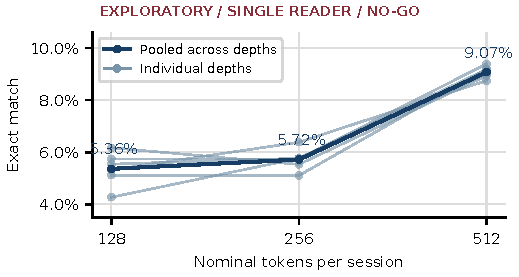
\includegraphics[width=\linewidth]{figures/fig2_em_by_budget_b.pdf}
\caption{Exact match by per-session budget $B\in\{128,256,512\}$ on 8,444 answerable non-refusal trials. Pooled rates rise from 5.36\% at $B=128$ to 9.07\% at $B=512$; the GEE budget coefficient is $+0.3166$ log-odds ($p=2.46\times10^{-4}$), with a positive budget response at every pilot depth $K$. Stamped: EXPLORATORY / SINGLE READER / NO-GO.}
\label{fig:em_by_budget}
\end{figure}

\subsection{Budget and interaction estimates}

Pooled EM was 6.71\% (567/8,444). It increased from 5.36\% at $B=128$ to 5.72\% at $B=256$ and 9.07\% at $B=512$ (Fig.~\ref{fig:em_by_budget}). The regression budget coefficient represents the slope at the centered depth. The depth and interaction estimates are imprecise (Table~\ref{tab:gee_results}). The interaction CI crosses zero and extends above the planned-design MDE (Figs.~\ref{fig:heatmap} and~\ref{fig:interaction_mde}). With the pilot's question-clustered interaction SE of $0.0168$, its realised interaction MDE at 80\% power is $\approx2.8\times0.0168\approx0.047$ log-odds, above the planned study's simulated $0.0308$; the estimate $0.0111$ is $0.3602$ times that planned MDE, which applies to the planned study.

\begin{table}[!t]
\centering
\caption{Exploratory GEE estimates from run \texttt{r\_fast\_final} with reader Gemma-4-E4B-it: 8,444 observations in 470 question clusters; SE is question-clustered.}
\label{tab:gee_results}
\small
\setlength{\tabcolsep}{3pt}
\begin{tabular}{@{}lrrlr@{}}
\toprule
Term & Estimate & SE & 95\% CI & $p$ \\
\midrule
$\log_2 K$ & $-0.0331$ & 0.0529 & $[-0.1368,0.0707]$ & 0.532 \\
$\log_2 B$ & $+0.3166$ & 0.0864 & $[0.1473,0.4858]$ & 0.000246 \\
Interaction & $+0.0111$ & 0.0168 & $[-0.0217,0.0439]$ & 0.508 \\
\bottomrule
\end{tabular}
\end{table}

In a replay, model-based SEs for depth, budget, and interaction were 0.0606, 0.0559, and 0.0326, against question-clustered robust SEs of 0.0529, 0.0864, and 0.0168 (Table~\ref{tab:gee_results}). The two covariances need not move together: $M^{-1}$ assumes independent within-question residuals, whereas the cluster-robust $M^{-1}(\sum_q u_qu_q^\top)M^{-1}$ uses observed residual cross-products. Positive within-question correlation inflates the robust SE (budget: 0.0864 vs 0.0559); negative or weak correlation shrinks it (depth: 0.0529 vs 0.0606; interaction: 0.0168 vs 0.0326). The direction is term-specific. Table~I uses question-clustered robust SEs throughout. The preference stratum exhibited separation (0/539 exact matches). Dropping that stratum left the three estimates and robust SEs unchanged to four decimal places. An extreme-bounds sensitivity analysis assigned the 16 excluded answerable refusals either all incorrect or all correct. Pooled EM ranged from 6.70\% to 6.89\%, and the budget coefficient ranged from 0.3166 to 0.3196 log-odds. A quasi-likelihood-ratio test on one degree of freedom compared the linear-in-$\log_2 K$ fit with a $(\log_2 K)^2$ term: quasi-LR $=0.1595$ ($p=0.6896$, $\hat\beta_{K^2}=-0.0202$). Curvature was not rejected within $K\le32$, but the $6.71\%$ exact-match floor leaves this functional-form check low-powered; the surface is not shown to be flat.

\begin{figure}[!t]
\centering
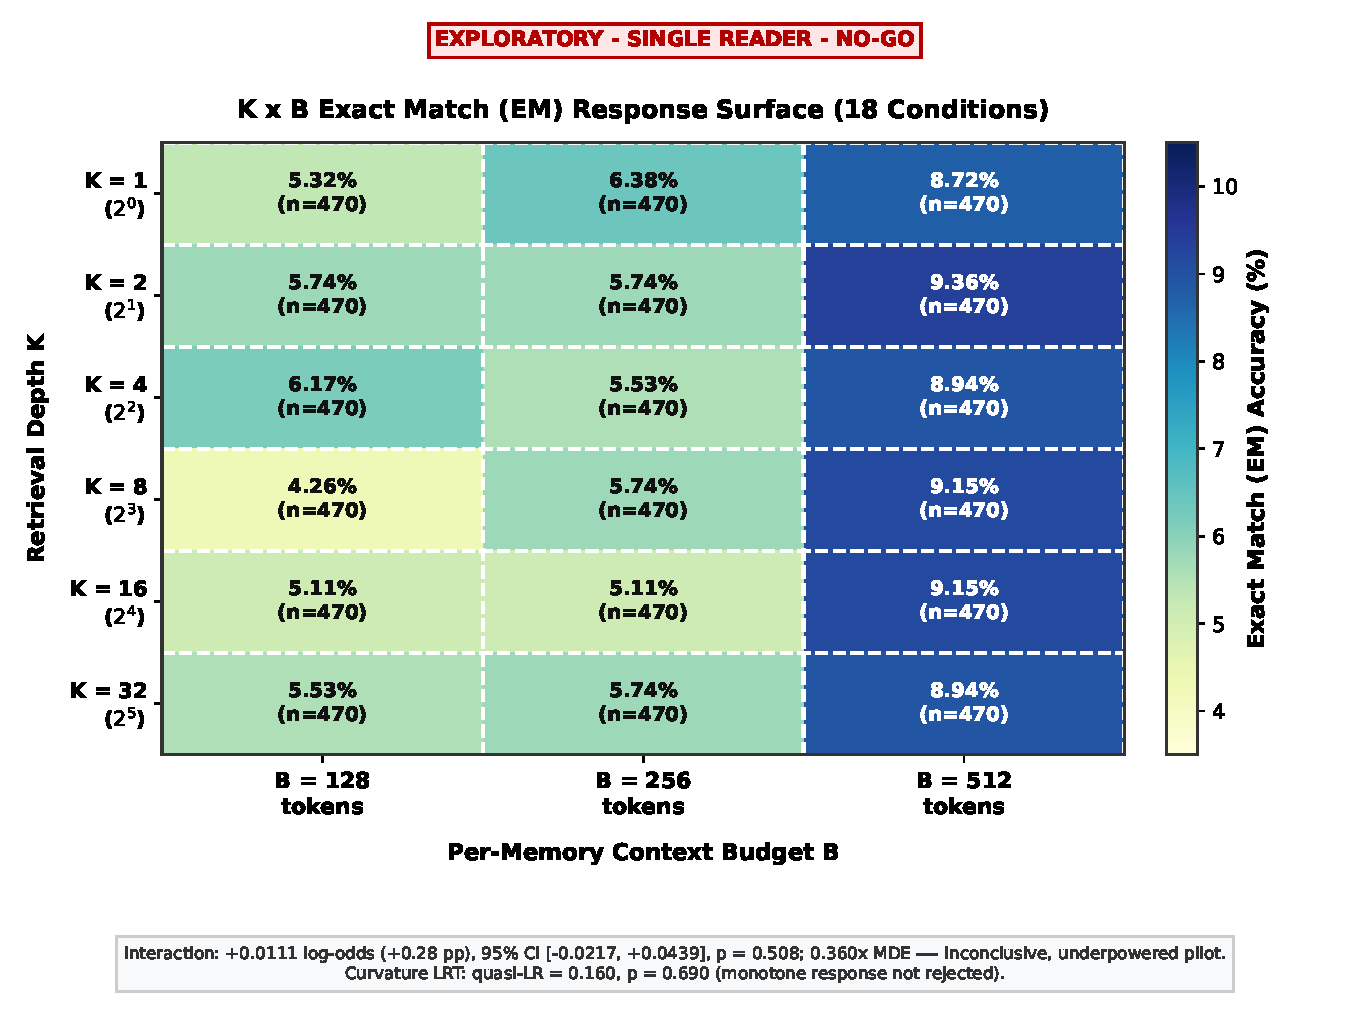
\includegraphics[width=\linewidth]{figures/fig3_kb_em_heatmap.pdf}
\caption{Exact-match rates in the 18 crossed $K\times B$ cells, with roughly 470 answerable trials per cell (excluding the 16 answerable refusals). The interaction estimate is $+0.0111$ log-odds ($p=0.508$, 95\% CI $[-0.0217,+0.0439]$), or $0.3602\times$ the planned $0.0308$ MDE. Stamped: EXPLORATORY / SINGLE READER / NO-GO.}
\label{fig:heatmap}
\end{figure}

\begin{figure}[!t]
\centering
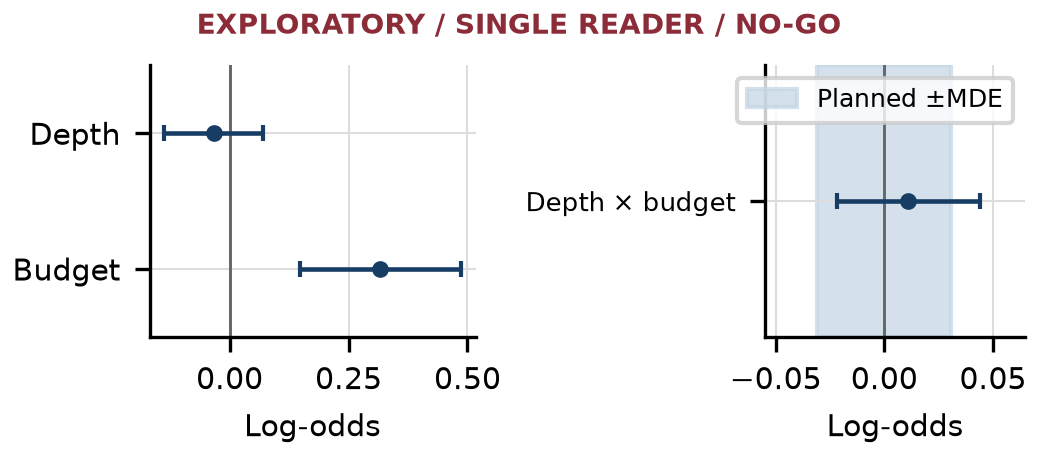
\includegraphics[width=\linewidth]{figures/fig4_interaction_estimate_mde.png}
\caption{Exploratory GEE estimates with 95\% cluster-robust Wald intervals. The interaction is $+0.0111$ log-odds ($+0.28$ pp at $p=0.5$), 95\% CI $[-0.0217,+0.0439]$, $p=0.508$; the shaded $\pm0.0308$ MDE band gives a ratio of $0.3602\times$. The budget coefficient is positive ($+0.3166$). Stamped: EXPLORATORY / SINGLE READER / NO-GO.}
\label{fig:interaction_mde}
\end{figure}

\subsection{Question types and latency}

Assistant-session EM dropped from 22.02\% at $K=1$ to 17.26\% at $K=32$ (Fig.~\ref{fig:em_by_k_ability}). Multi-session EM stayed between 0.28\% and 1.11\% across depths (14 exact matches in 2,172 trials). The accuracy floor and the strict scoring rule limit what these differences can establish about attention, retrieval rank, or usefulness of larger budgets.

\begin{figure*}[!t]
\centering
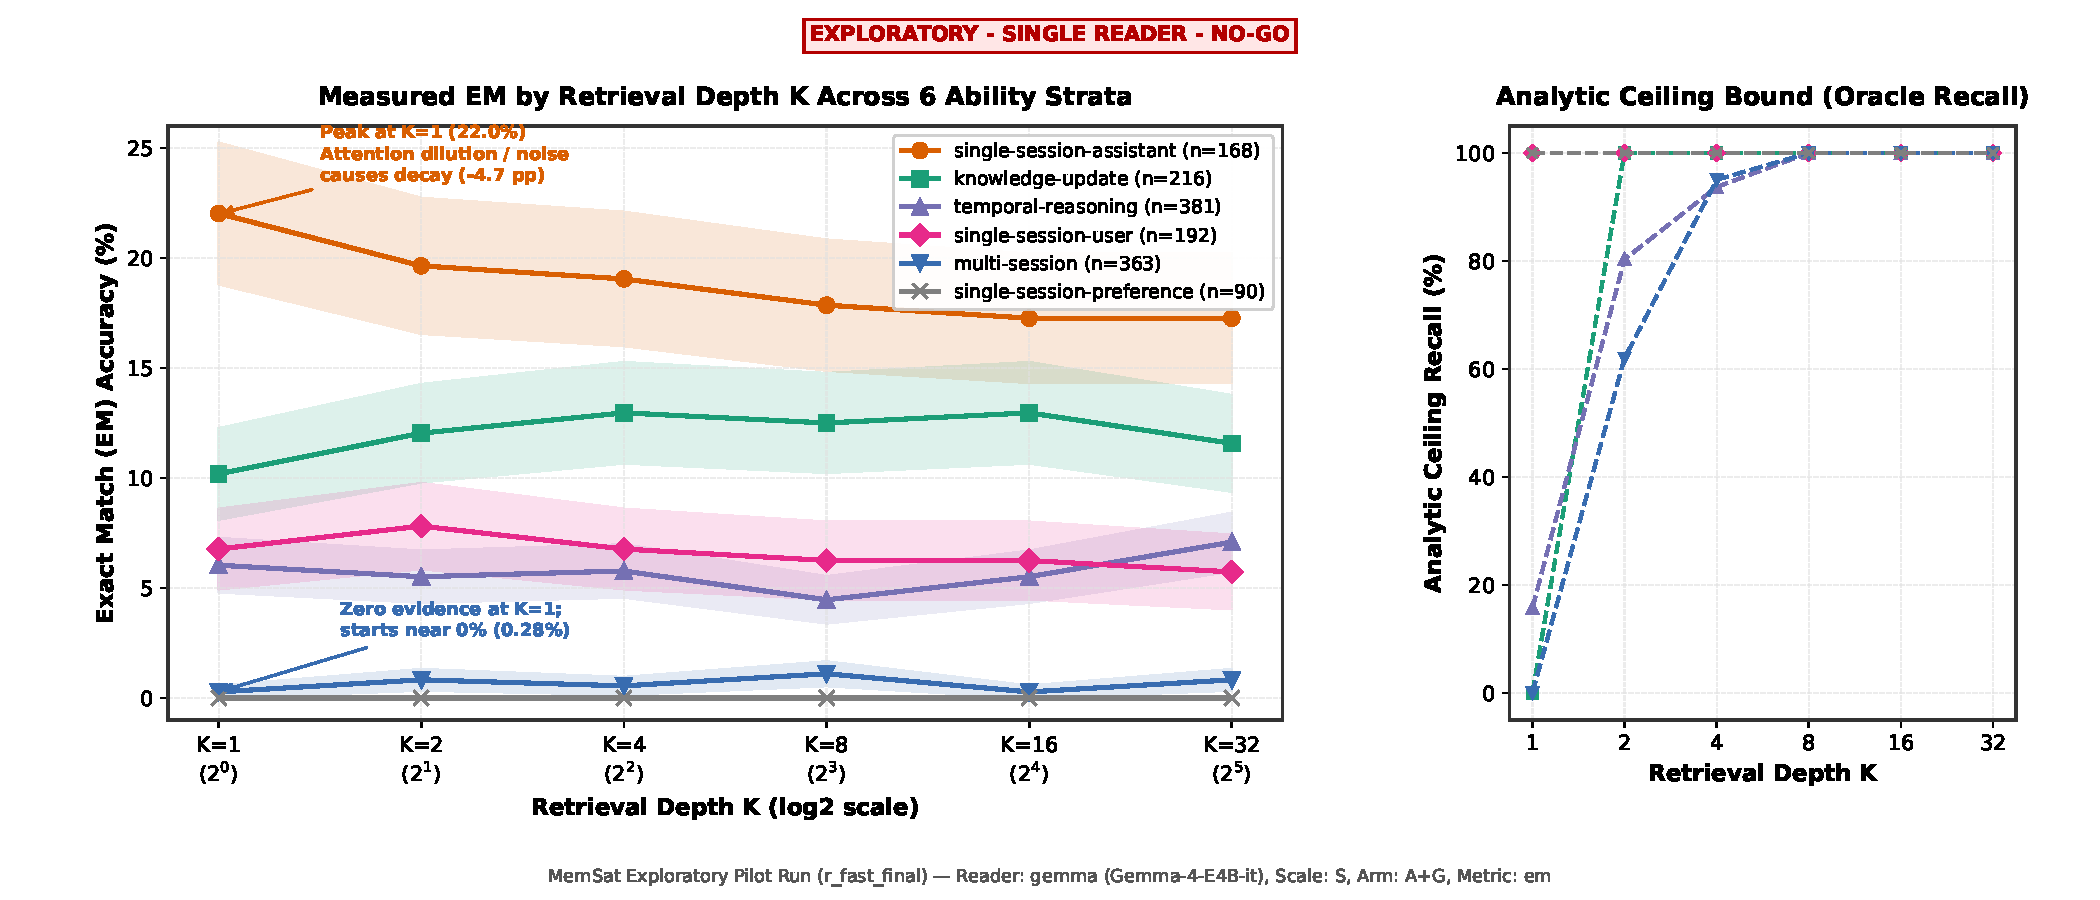
\includegraphics[width=\textwidth]{figures/fig5_em_by_k_ability.pdf}
\caption{Exact match by depth and question type for 8,444 answerable non-refusal trials. Left: measured EM across six ability strata; right: the corresponding analytic ceiling bound. Single-session-assistant items fall from about 22.0\% at $K=1$ to 17.3\% at $K=32$, while multi-session items stay at or below 1.1\%. Stamped: EXPLORATORY / SINGLE READER / NO-GO.}
\label{fig:em_by_k_ability}
\end{figure*}

Across 9,004 latency records on a laptop RTX 4060, median generation time was 6.62~s (IQR 3.81~s), 95th percentile 15.72~s; crossed trials rose from 5.87 to 7.85~s between $B=128$ and $B=512$, with IQR 2.74 to 6.04~s (Fig.~\ref{fig:latency_dist}). For 2,000 crossed trials at $K\ge4$, $B=512$, the pooled 95th percentile was 26.15~s. By nominal budget, the 95th percentile rose from $10.70$~s at $B=128$ to $12.97$~s at $B=256$ and $22.95$~s at $B=512$; observations spanned $2.83$--$70.63$~s. These descriptive tails are distinct from the pooled $15.72$~s and crossed $26.15$~s figures and share the prefill-chunk confound. The backend timed post-tokenization generation, covering prefill and decoding; for this backend, time to first token would run from the start of packed-prompt prefill to the first emitted token and was not recorded. A 512-token prefill chunk setting was recorded on 7,341 trials and blank on 1,663, confounding the budget--latency comparison: with prefill unmeasured, the median rise with $B$ cannot be attributed to budget alone.

\begin{figure*}[!t]
\centering
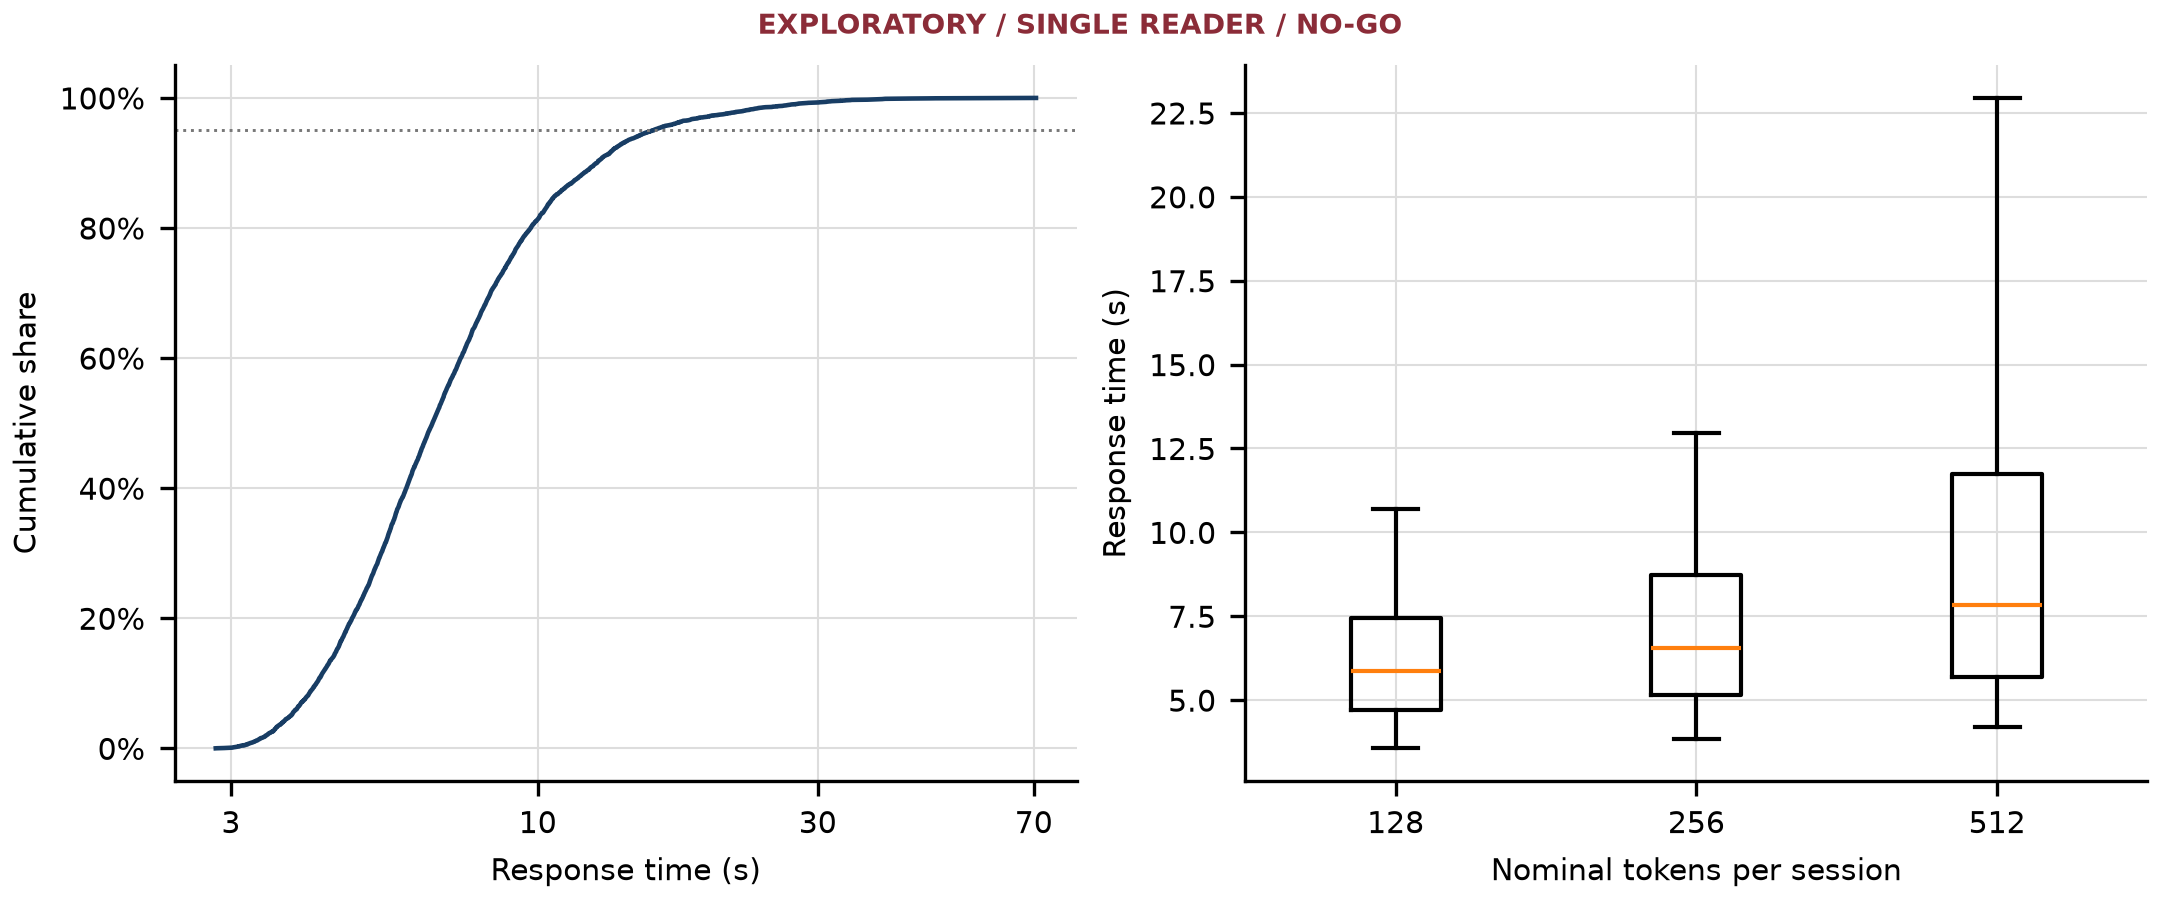
\includegraphics[width=0.85\textwidth]{figures/fig6_latency_distribution.png}
\caption{Response-time distribution for 9,004 records on a laptop RTX 4060 (median 6.62~s, IQR 3.81~s, $p90=12.59$~s, $p95=15.72$~s), with the 9,000 crossed trials broken down by nominal budget; dispersion roughly doubles across $B$. Quartiles and tail percentiles are descriptive. Stamped: EXPLORATORY / SINGLE READER / NO-GO.}
\label{fig:latency_dist}
\end{figure*}

\section{Discussion and Limitations}

The benchmark supplies a depth diagnostic from pre-truncation metadata, not deployment policy: it bounds retrievable sessions, not reader use. An oracle recovers all gold sessions for single-session questions at $K=1$, but observed top-1 recall varies by type. A policy with $K=1$ and a confidence-based fallback is a testable proposal, not a mandate from the ceiling; on multi-session questions $K=1$ cannot recover all labeled sessions. More $K$ can recover evidence when retrieval is imperfect even beyond oracle saturation. Whether more of each session helps the reader use distributed evidence needs a less floor-limited evaluation.

The pilot is limited to one quantized reader, one retriever, one scale, and one offline scoring metric. Truncation can remove evidence from a retrieved session, and observed rank is partly determined by $K$ and retrieval success. A prospective analysis should specify whether it estimates the total effect of changing the factors or an association conditional on rank. The unanswerable trials require separate abstention evaluation. Statistical uncertainty in the interaction and the absence of cross-reader results preclude a general conclusion about its magnitude or sign.

For homogeneous full-attention layers with $H_{\rm KV}$ key/value heads of dimension $d$, a 16-bit cache uses approximately $4LH_{\rm KV}d$ bytes per input token across $L$ layers. Applied to the planned reader panel, this model gives roughly 82--375~MB per 1,000 tokens; hybrid or shared caches, placement, and allocation overhead change the estimate, so this is a modeled figure that requires per-backend measurement. The measured tail times motivate evaluating retrieval policies within an explicit latency target. Techniques such as PagedAttention address KV-cache allocation~\cite{kwon2023pagedattention}. Their effects on this pipeline remain to be measured.

\section{Conclusion}

The cleaned LongMemEval releases support an oracle complete-recall ceiling of six sessions at the specified tolerance, with pronounced differences by question type --- an analytic dataset property before truncation, not operating guidance. The protocol-specified crossed depth--budget GEE remains unexecuted. The single-reader pilot found higher exact match at larger budgets amid severe scoring floors and higher latency, but it is exploratory, halted at a NO-GO gate, and strict full-string exact match can reward longer outputs, so the association is not evidence of better evidence quality. Its interaction estimate leaves a range of plausible effects, and the coverage gate stopped advancement. The results establish a benchmark diagnostic and specify what a confirmatory study must measure.

\section*{Data and Code Availability}
The benchmark is the cleaned LongMemEval release at revision \texttt{98d7416}. The analysis harness is available from the authors upon reasonable request. The companion package (\texttt{paper/reproduction/}) includes derived question and pilot records, gate and power summaries, and a script to replay the analyses and figures.

% REFERENCES start on a fresh final page.
\newpage
\begin{thebibliography}{27}
\scriptsize

\bibitem{lewis2020rag}
P.~Lewis \emph{et~al.}, ``Retrieval-augmented generation for knowledge-intensive NLP tasks,'' in \emph{Advances in Neural Information Processing Systems (NeurIPS)}, vol.~33, pp.~9459--9474, 2020, doi: 10.48550/arXiv.2005.11401.

\bibitem{packer2023memgpt}
C.~Packer, S.~Wooders, K.~Lin, V.~Fang, S.~G. Patil, I.~Stoica, and J.~E. Gonzalez, ``MemGPT: Towards LLMs as operating systems,'' \emph{arXiv preprint arXiv:2310.08560}, 2023, doi: 10.48550/arXiv.2310.08560.

\bibitem{wu2025longmemeval}
D.~Wu, H.~Wang, W.~Yu, Y.~Zhang, K.-W. Chang, and D.~Yu, ``LongMemEval: Benchmarking chat assistants on long-term interactive memory,'' in \emph{International Conference on Learning Representations (ICLR)}, 2025, arXiv:2410.10813, doi: 10.48550/arXiv.2410.10813.

\bibitem{maharana2024locomo}
A.~Maharana, D.-H. Lee, S.~Tulyakov, M.~Bansal, F.~Barbieri, and Y.~Fang, ``Evaluating very long-term conversational memory of LLM agents,'' in \emph{Proceedings of the 62nd Annual Meeting of the Association for Computational Linguistics (Volume 1: Long Papers)}, pp.~13851--13870, 2024, doi: 10.18653/v1/2024.acl-long.747.

\bibitem{huang2026licomemory}
Z.~Huang \emph{et~al.}, ``LiCoMemory: Lightweight and cognitive agentic memory for efficient long-term reasoning,'' in \emph{Findings of ACL}, pp.~36842--36858, 2026, doi: 10.18653/v1/2026.findings-acl.1835.

\bibitem{yuan2026diagnosing}
B.~Yuan, Y.~Su, and K.~Yao, ``Diagnosing retrieval vs. utilization bottlenecks in LLM agent memory,'' in \emph{ICLR 2026 Workshop on Memory for LLM-Based Agentic Systems (MemAgents)}, 2026, arXiv:2603.02473, doi: 10.48550/arXiv.2603.02473.

\bibitem{shao2026storedevidence}
J.~Shao, Y.~Lu, Y.~Zhang, and B.~Luo, ``When stored evidence stops being usable: Scale-conditioned evaluation of agent memory,'' \emph{arXiv preprint arXiv:2605.07313}, 2026, doi: 10.48550/arXiv.2605.07313.

\bibitem{shen2026evictiondestroys}
C.~Shen, ``What eviction destroys: A restore-counterfactual audit of forgetting in agent memory,'' \emph{arXiv:2609.08279}, 2026, doi: 10.48550/arXiv.2609.08279.

\bibitem{sidik2026memtier}
B.~Sidik and L.~Rokach, ``MEMTIER: Tiered memory architecture and retrieval bottleneck analysis for long-running autonomous AI agents,'' \emph{arXiv:2605.03675v3}, 2026.

\bibitem{zhou2026reproducinglightmem}
Y.~Zhou, S.~Wang, B.~Koopman, and G.~Zuccon, ``Reproducing LightMem: When does memory construction help over raw-turn retrieval?'' \emph{arXiv:2607.29104v2}, 2026.

\bibitem{liu2026evalmem}
Z.~Liu \emph{et~al.}, ``EvalMem: An operation-level diagnostic framework for long-term memory systems,'' in \emph{Findings of EMNLP}, pp.~24002--24034, 2026, doi: 10.18653/2026.findings-emnlp.1134.

\bibitem{yu2026whenloss}
J.~Yu, K.~S. Lin, and J.~Wu, ``WhenLoss: Diagnosing write and retrieval bottlenecks in long-context memory systems,'' \emph{arXiv preprint arXiv:2605.24579}, 2026, doi: 10.48550/arXiv.2605.24579.

\bibitem{kang2026retainconsolidate}
Q.~Kang, M.~Liu, S.~Kai, K.~Liang, Z.~Tang, Y.~Cui, T.~Zhong, and M.~Yuan, ``Retain or consolidate? Budget-dependent operator selection for language agent memory,'' \emph{arXiv preprint arXiv:2607.17545}, 2026, doi: 10.48550/arXiv.2607.17545.

\bibitem{andreev2026depthwidth}
M.~Andreev, ``Memory depth and reconstructed context width: A controlled evaluation of hierarchical retrieval,'' \emph{arXiv:2610.08300}, 2026, doi: 10.48550/arXiv.2610.08300.

\bibitem{levy2025moredocuments}
S.~Levy, N.~Mazor, L.~Shalmon, M.~Hassid, and G.~Stanovsky, ``More documents, same length: Isolating the challenge of multiple documents in RAG,'' in \emph{Findings of EMNLP}, pp.~19539--19547, 2025, doi: 10.18653/v1/2025.findings-emnlp.1064.

\bibitem{liu2024lostmiddle}
N.~F. Liu, K.~Lin, J.~Hewitt, A.~Paranjape, M.~Bevilacqua, F.~Petroni, and P.~Liang, ``Lost in the middle: How language models use long contexts,'' \emph{Transactions of the Association for Computational Linguistics}, vol.~12, pp.~157--173, 2024, doi: 10.1162/tacl\_a\_00638.

\bibitem{hong2025contextrot}
K.~Hong, A.~Troynikov, and J.~Huber, ``Context rot: How increasing input tokens impacts LLM performance,'' \emph{Chroma}, Technical Report, 2025.

\bibitem{systems2026ragstability}
B.~S.~R.~Muthyam, ``A systems-level analysis of sensitivity, robustness, and stability in retrieval-augmented generation,'' \emph{arXiv:2606.28337}, 2026, doi: 10.48550/arXiv.2606.28337.

\bibitem{panthi2026fixedrag}
S.~Panthi and R.~Abdelfattah, ``Compression is not evaluation-neutral: Fixed RAG compression can distort reader comparisons,'' \emph{arXiv:2606.21807v2}, 2026.

\bibitem{chanhnourack2026auditing}
C.~J. Chanhnourack, ``Auditing long-term memory evaluation: Repeated judging, reader variation, and negative controls,'' \emph{arXiv preprint arXiv:2609.38021}, 2026, doi: 10.48550/arXiv.2609.38021.

\bibitem{liu2025kappa0118}
J.~Liu, H.~Qiu, J.~Lasko, D.~Karakos, M.~Yarmohammadi, and M.~Dredze, ``Demo: Statistically significant results on biases and errors of LLMs do not guarantee generalizable results,'' \emph{arXiv preprint arXiv:2511.02246}, 2025, doi: 10.48550/arXiv.2511.02246.

\bibitem{landis1977measurement}
J.~R. Landis and G.~G. Koch, ``The measurement of observer agreement for categorical data,'' \emph{Biometrics}, vol.~33, no.~1, pp.~159--174, 1977, doi: 10.2307/2529310.

\bibitem{zhang2026budgetmem}
H.~Zhang \emph{et~al.}, ``Learning query-aware budget-tier routing for runtime agent memory,'' in \emph{Proc. ICML}, PMLR, vol.~306, pp.~160227--160264, 2026.

\bibitem{denning1968workingset}
P.~J. Denning, ``The working set model for program behavior,'' \emph{Commun. ACM}, vol.~11, no.~5, pp.~323--333, 1968, doi: 10.1145/363095.363141.

\bibitem{article2018preregistration}
B.~A. Nosek, C.~R. Ebersole, A.~C. DeHaven, and D.~T. Mellor, ``The preregistration revolution,'' \emph{Proceedings of the National Academy of Sciences}, vol.~115, no.~11, pp.~2600--2606, 2018, doi: 10.1073/pnas.1708274114.

\bibitem{liang1986longitudinal}
K.-Y. Liang and S.~L. Zeger, ``Longitudinal data analysis using generalized linear models,'' \emph{Biometrika}, vol.~73, no.~1, pp.~13--22, 1986, doi: 10.1093/biomet/73.1.13.

\bibitem{kwon2023pagedattention}
W.~Kwon \emph{et~al.}, ``Efficient memory management for large language model serving with PagedAttention,'' in \emph{Proc. SOSP}, 2023, doi: 10.1145/3600006.3613165.

\end{thebibliography}
